\documentclass[11pt,a4paper,twoside,openright]{report}

\usepackage{algpseudocode,algorithm}	
\usepackage{listings}
\usepackage{amsmath,amssymb}  
\usepackage{graphicx}
\usepackage{tabularx}
\usepackage{subfigure}
\usepackage{afterpage}          
\usepackage{rotating}  
\usepackage{fancyhdr}  
\usepackage[scriptsize]{caption} 
\usepackage{seqsplit}
\hyphenation{a-gen-tiz-za-zio-ne}

\setlength{\paperwidth}{16cm}
\setlength{\paperheight}{24cm}
\setlength{\oddsidemargin} {2. cm}
\setlength{\evensidemargin} {2. cm}
\addtolength{\oddsidemargin} {-0.4 cm}
\addtolength{\evensidemargin} {-0.4 cm}
\linespread{1.1}

\usepackage[english]{babel}
\usepackage[latin1]{inputenc}
\renewcommand{\captionfont}{\normalfont \sffamily \itshape \small}

\pagestyle{empty}

\begin{document}
\thispagestyle{empty}
%\begin{titlepage}
\vspace*{-1.5cm} \bfseries{
\begin{center}
  \large
  POLITECNICO DI MILANO\\
  \normalsize
  Dipartimento di Elettronica, Informazione e Bioingegneria\\
  
  \vspace*{0.5cm}
  
  \begin{figure}[htbp]
    \begin{center}
      
\includegraphics[width=4cm]{images/polimi.png}
    \end{center}
  \end{figure}
  \vspace*{0.3cm} 
  
  \LARGE
  \textbf{SPF2}\\
  Social Proximity Framework 2\\

  \vspace*{.75truecm} \large
  DEEP-SE \\
  DEpendable Evolvable Pervasive\\
  Software Engineering
\end{center}
\vspace*{3.0cm} \large
\begin{flushleft}

  %Relatore: Prof. \\
  %Correlatore: Prof. 

\end{flushleft}
\vspace*{1.0cm}
\begin{flushright}


  Author:\\ 
  Stefano CAPPA

\end{flushright}
\vspace*{0.5cm}
\begin{center}

  %Anno Accademico 2014-2015
\end{center} \clearpage
}


\thispagestyle{empty} \normalfont \cleardoublepage

% ---- Page header setup ----
\pagestyle{plain}\renewcommand{\chaptermark}[1]{\markboth{\chaptername\ \thechapter.\ #1}{}} 
\renewcommand{\sectionmark}[1]{\markright{\thesection.\ #1}}         
\fancyhead[LE,RO]{\bfseries\thepage}      
\fancyhead[RE]{\bfseries\leftmark}
\fancyhead[LO]{\bfseries\rightmark}     
\renewcommand{\headrulewidth}{0.3pt} 


% ---- Table of contents ----
\tableofcontents
\listoffigures
\lstlistoflistings
\cleardoublepage

\pagenumbering{arabic}
\setcounter{page}{1}

% ---- Chapters ----
\chapter{Introduction}
\label{chap1}

This document describes SPF2 (Social Proximity Framework 2), the new major release of the software written for the master thesis available at http://hdl.handle.net/10589/106727. Before you could understand this document you must really read the first one. This document will be more implementation-level then the master thesis and for this reason i won't repeat the theory behind SPF.

The main objectives of this second major release are:
\begin{itemize}
	\item update the entire project to Android Studio and Gradle;
	\item split the 3 demo applications in different projects;
	\item put SPFShared and SPFLib into a Maven repository to be able to import in all project what you want to create SPF's applications;
	\item update all GUIs to Material Design and in particular using the necessary support library by Google
	\item officially support Android 6.0
	\item completely remove AllJoyn/AllSeen middleware and replace it with a pure and complete Wi-Fi Direct middleware
	\item improve Wi-Fi Direct Middleware's architecture and sourcecode improving the reliability
	\item support Wi-Fi Direct groups made by 2 or more devices
\end{itemize}

But why I chose this particular objectives? Because, I decided to:
\begin{itemize}
	\item To update the project to the news Android's IDE and its build tool, because Google decided to stops the development of ADT for Eclipse
	\item To improve the separation of concepts and the related projects
	\item To simplify the usage of SPF by app's developers
	\item To simplify the future work from SPF developers to add other GUI elements and so on \dots In fact, updating all projects to support library will make easier to update SPF to newer Android versions and Themes.
	\item To use the Wi-Fi Direct protocol, created exactly for mobile devices
	\item To use my previous experiences working on Wi-Fi Direct to improve the stability and reliability of Wi-Fi Direct middleware
	\item To support Wi-Fi Direct groups specifying from the UI which type of device will be after the Proximity service will be enabled
\end{itemize}

All projects are available on GitHub licensed under LGPLv3 and I also included Travis Continuous Integration to auto compile the source code at every \textsf{git push} command, in particular to check the different releases.
The official repositories are:
\begin{enumerate}
	\item https://github.com/deib-polimi/SPF2
	\item https://github.com/deib-polimi/SPF2CouponingProviderDemo
	\item https://github.com/deib-polimi/SPF2CouponingClientDemo
	\item https://github.com/deib-polimi/SPF2ChatDemo
\end{enumerate}
The first one is the main project, with also SPFShared and SPFLib. In this project all sub-modules are connected using normal gradle module's dependency.
I.e. there is a settings.gradle file where are declared all submodules and
in every local module's build.gradle are specified the dependency from other sub module.
For example, this is the settings.gradle
include ':sPFShared'
include ':sPFFramework'
include ':sPFWFDMid'
include ':sPFLib'
include ':sPFApp'


and this one is the build.gradle in sPFFramework sub module:
dependencies {
    compile \seqsplit{project(':sPFShared')}
    compile \seqsplit{'com.google.code.gson:gson:2.4'}
    compile \seqsplit{'com.android.support:support-v4:23.1.0'}
    provided \seqsplit{'org.projectlombok:lombok:1.16.6'}
}

As you can see there are local module's dependencies like gson and support-v4, a provided dependency like lombok and finally the dependency of sPFShared module, not online like the others, but local into the Android Studio Project. In fact, all the dependencies in SPFApp are local because it's the place where you can develop their. In external apps, like SPFCouponing and SPFChat, all dependencies are remote, using the deployed version of SPFShared and SPFLibs. This is the correct way to manege dependencies for SPF.
A very big improvement should be the total separation of SPFApp from sPFFramework and all other sub modules. But this is another topics and i will show more details and hints at the end of this document, because should be the main objective for the next major release.

\section{The new project structure}
After the first overview it's time to explain in detail the new project structure for SPFApp. Like described before, all applications based on SPF should only add the maven dependencies for SPFShared and SPFLib.

\section*{sPFApp module}

For main project, the structure is more complicated.
There is an Android application called SPFApp, that it's the main module, because in its gradle file there is this line: ``apply plugin: 'com.android.application'``.
In this file i specify some informations, like versionCode and versionName. These two values are important, because when you want to release another version you should increase the versionCode and change the versionNane, for example ``3.0.0`` or ``2.1.0``.
An important part to mantain updated this application is to force the compileSdkVersion, buildToolsVersion and targetSdkVersion to the latest available values. Also, it's a good practice to always use the latest gradle wrapper, forcing the version into all gradle files n this way:

task wrapper(type: Wrapper) {
    gradleVersion = "2.8"
}

But, the most important part are the dependencies.
Inside this block there are all the local dependencies for this module. In particular, for SPFApp, the list is very long, because there are all the library to create the gui, like MaterialDrawer, Iconics, Butterknife, CircleImageView, Soundcloud-crop.
It's very important to always update this libraries because some of them receive a huge amount of updates with fixes and improvements.
Also, there other dependencies like Lombok to use annotations like @Getter and @Setter.
At the moment, Lombok require a config file called lombok.config to be able to build the project.

Finally there are all the google dependencies to be able to target different Android versions using the latest gui componenets. Remember to use classes from the support libraries to be able to show the latest and modern gui  elements in all Androids version, when it's possibile. For example use Fragment class from appcompat-v4, or AppCompatActivity and not simply Activity, or Loader and AsyncTaskLoader from appCompatv7 and so on. I you follow this simple suggestions the next updates of this  will be very simple.
Also remember to choose the correct Android Theme in src/res/values/styles.xml, like Theme.AppCompat.Light.NoActionBar. This is absolutely required by Android when you want to use supports libraries.

Finally, to be able to compile with Travis CI, you must provide the correct .travis.yml file specifying exactly the same version written in you gradle files.
For example, if you are targeting API 23, into your travis file you must write 
- android-23

But, where are all the dependencies described here? They are on Maven Central Repository. This means that they are online or local if you have previously downloaded those files.
The dependencies specified with ``compile project(':moduleName')`` are the local modules into the AndroidStudio Project. Obviously, this means that are local.

\section*{sPFFramework and sPFWFDMid modules}
These are ``com.android.library`` module. For this reason, you can't start they as Android Applications.
The structure is quite the same, always with remote and local dependencies.

\section*{sPFLib and sPFShared modules}
These are different modules, because have also ``apply plugin: 'maven'`` to be able to push on a local Maven Server on your PC.
In my case, I chose \emph{Sonatype Nexus OSS} and i specified inside these two build.gradle files the uploadeArchives task to be able to push on the local server the compiled libraries and to use inside another different Android project that request these files.
This is very useful during development. In this way you aren't oblied to push all snapshots version into a remove maven repository, but you can test your code locally.
To be able to use this you must download the server from http://www.sonatype.org/nexus/go/. 
After tht start the server following the informations on the official websites and you can enter with http://localhost:8081/nexus and login as administrator.
To be able to push directly to this serve to AndroidStudio the only thing that you must do is:
create a gradle.properties inside the root project and put this inside:

nexusUrl=http://localhost:8081/nexus
nexusUsername=admin
nexusPassword=admin123

Remember to not push this file remotely, this should be only a local configuration for your machine.

After that, build the entire project and now you are able to upload SPFLib and SPFShared into this server executing from Android Studio the uploadArchives task into these two projects. Remember that at every upload you should increace the version number into the build.gradle or you should remove the folder inside you server.

With this informations you can build SPFApp, but what you should do if you want to build SPF external applications that require SPFShared and SPFLib?
If you want to use my stable versions, you can simply follow the procedure described at the start of this section, but which is the correct procedure to use the versions from Sonatype Nexus OSS?
It's very simple, because you should use this main build.gradle file:

\begin{lstlisting}
	
// Top-level build file
buildscript {
  repositories {
  jcenter()
  maven {
    url "http://localhost:8081/nexus/
    	  content/groups/public"
  }
  }
  dependencies {
    classpath 'com.android.tools.build:gradle:1.3.1'
  }
}

allprojects {
  repositories {
    jcenter()
    maven {
      url "http://localhost:8081/nexus/
      		content/groups/public"
    }
  }
}
\end{lstlisting}

Yes, also in this file you should always update the gradle build tools, to be able to use all latest libraries and functions of the IDE (for example in the future Android Data Binding will be relased, and to be able to use this, you will must update the build tools to compile, the same happened some months ago with the NDK support).

After that, you can simply put these dependencies:

compile 'it.polimi.spf:spflib:2.0.0.0@aar'
compile 'it.polimi.spf:spfshared:2.0.0.0@aar'


into your local build.gradle file into your SPF application.

Obviously, to be able to compile, Sonatype Nexus OSS must be running with this files. 

With all these informations you can simply build all your SPF applications and updates all dependencies and tools to the latest versions.




\chapter{Wi-Fi Direct Middleware}
\label{chap2}
\thispagestyle{empty}

\noindent In this section I'll show the low-level architecture of the sPFWFDMid module. With this chapter you'll able to update the middleware in the future. Because, I have completely changed most of the code in this module, you should consider completely deprecated the version of SPF1 and the related documentation.

\section{A quick overview}

All Wi-Fi Direct Middleware are into the sPFWFDMid sub-module. There are two main packages:

\begin{itemize}
	\item wfd: contains the entire logic 
	\item wfdadapter: contains all the classes and interfaces directly related to SPF
\end{itemize}

When you open SPF on your smartphone, the first thing that happens, also before the start of the MainActivity, is the execution of the code into the SPFApp.java, that extends Application. 
The first thing that SPFApp does is inside its Application's class, where there is the initialization of SPF, with this line \textsf{SPFContext.initialize(this, 0, true, WFDMiddlewareAdapter.FACTORY);}. As you can see, the only things that you must provide to this method are:
\begin{itemize}
	\item \textsf{context}: necessary to use all methods that require context into the middleware, where there aren't any ways to get it.
	\item \textsf{goIntent} and \textsf{isAutonomous}: are specific for Wi-Fi Direct Middleware. I'll talk on that during this document. Obviously, it should be removed in the future.
	\item \textsf{middleware}: to specify the middleware that you want to use. In SPF2, the only available middleware is Wi-Fi Direct.
\end{itemize}


\begin{figure}[thpb]
	\centering
	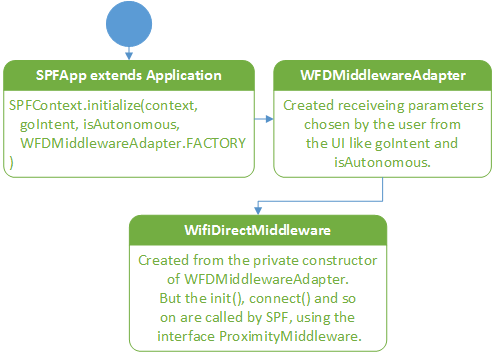
\includegraphics[scale=0.5]{./images/chap2/uml-parte0-1.png}
	\caption{General flow from SPFApp to the middleware}
	\label{uml-part0-1}
\end{figure}	

After that, as you can see in Figure \ref{uml-part0-1}, WFDMiddlewareAdapter (the most important class included into the \textsf{wpdadapter}'s package of the middleware) will be created and automatically it will instantiate the \textsf{WifiDirectMiddleware} object (the most important class included into the \textsf{wfd}'s package of the middleware). This process completes only with the creation of this last object, because the real initialization process and connection are made by SPF using the \textsf{ProximityMiddleware} interface. I'll discuss more in details these aspects during this session.
At the moment, i want explain only the events used to send messages into the middleware. The main idea was to prevent most of the cyclic dependencies that Wi-Fi Direct APIs force to use. To do that I used a library called Otto. 
Otto is an event bus designed to decouple different parts of your application while still allowing them to communicate efficiently. Forked from Guava, Otto adds unique functionality to an already refined event bus as well as specializing it to the Android platform.
To be able to post events in all Threads, I used a wrapper called Ninebus.
But, the only difficulties to use this library is how maintain an ordered structure. 

\begin{figure}[thpb]
	\centering
	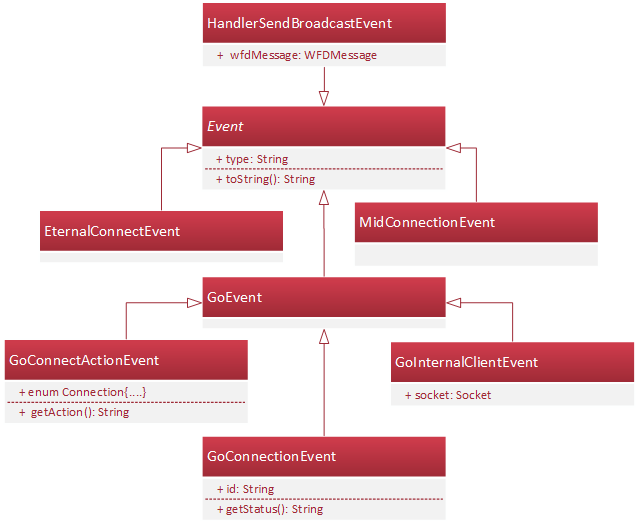
\includegraphics[scale=0.7]{./images/chap2/event-hyerarchy.png}
	\caption{Uml part 0.}
	\label{event-hyeranchy}
\end{figure}	

\begin{figure}[thpb]
	\centering
	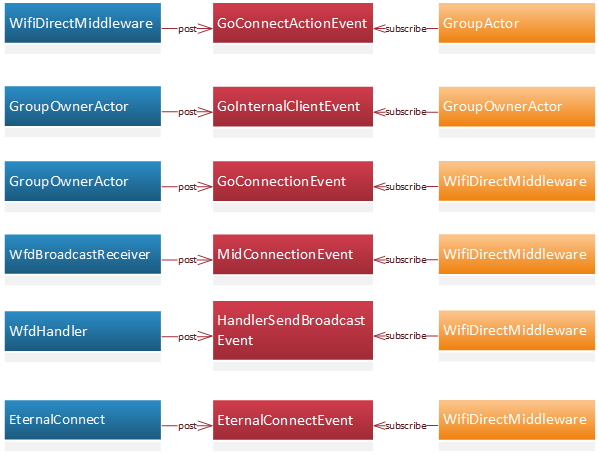
\includegraphics[scale=0.7]{./images/chap2/event-subscribe-post.png}
	\caption{Event post/subscribe responsibilities}
	\label{event-subscribe-post}
\end{figure}	

To achieve this, I used a package with all events inside, organized using the Java hierarchy. The complete class diagram of all events is in Figure \ref{event-hyeranchy}.
Another important thing is to understand which class posts an event and which will react its. To exmplain in a very simple way this fact, I created the diagram in Figure \ref{event-subscribe-post}. As you can see:
\begin{itemize}
	\item the blue elements are the classes the post events;
	\item in red there are all events;
	\item in orange are represented all subscribers.
\end{itemize}

This means that, \textsf{WifiDirectMiddleware.java} posts a \textsf{GoConnectActionEvent} and \textsf{GroupActor} will catch the events and it will react to its, executing a method annotated with \textsf{@Subscribe}.

\section{Architecture}

\begin{figure}[thpb]
	\centering
	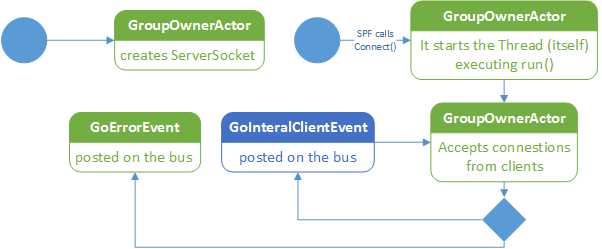
\includegraphics[scale=0.5]{./images/chap2/uml-parte0-2.png}
	\caption{GroupActor post behavior}
	\label{uml-part0-2}
\end{figure}	

\begin{figure}[thpb]
	\centering
	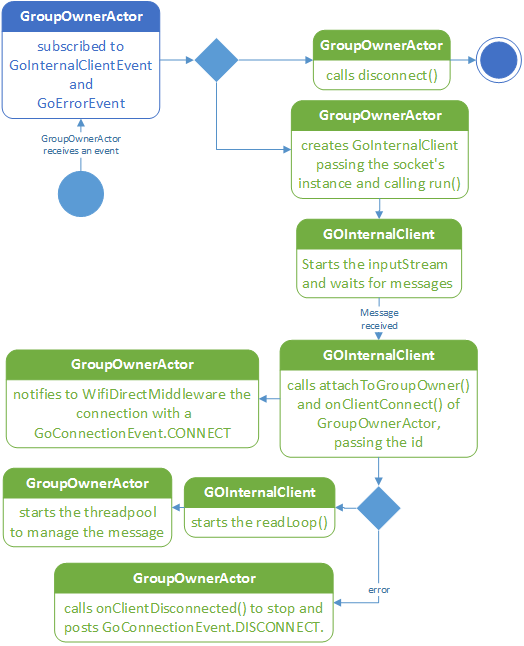
\includegraphics[scale=0.6]{./images/chap2/uml-parte0-3.png}
	\caption{GroupActor subscribe behavior}
	\label{uml-part0-3}
\end{figure}	

I don't want to explain in details the code of this middleware, instead, I want to explain the structure and the interactions of the classes inside the wfd/groups package.
I created two different scheme to describe this. They are represented as state diagram because very simple to read, but probably the best type of UML could be the Sequence Diagram.
First, I want to describe how \textsf{GroupActor} and its subclasses post events. As you can see in Figure \ref{uml-part0-2}, when \textsf{GroupOwnerActor} starts, it will create a \textsf{ServerSocket}, nothing more. It's SPF that calling the connect method will starts the \textsf{GroupOwnerActor}'s thread executing its \textsf{run()} method. Inside of its, it will start to listen and accept clients connections. If everything will be ok, it will post a \textsf{GoInternalClientEvent} on the bus, instead a \textsf{GoErrorEvent}. In the first case, it will return to listen and accepts other clients, forced by a while cycle. Obviously, this is only an extreme abstraction. To understand more in detail this, look the Figure \ref{uml-part0-3} where I represented the sequence of operations started when \textsf{GroupOwnerActor} receives the \textsf{GoInternalClientEvent} posted by itself (from is \textsf{run()} method and for this reason from another thread).
When \textsf{GroupOwnerActor} receives this event, it will create and starts a \textsf{GoInternalClient}, passing the socket instance. After that, this last thread starts the InputStream and waits for messages. 
When it receive a message, it calls \textsf{attachToGroupOwner()} and \textsf{onClientConnect()} of \textsf{GroupOwnerActor}, passing the identifier of the profile. These calls are necessary to notify to the \textsf{WifiDirectMiddlware} what happened, but the real logic will continue into the method \textsf{readLoop()} inside the \textsf{GoInternalClient} that start the threadpool into \textsf{GroupOwnerActor} to manage the message. All these operations written here are perfectly represented in Figure \ref{uml-part0-3}.


\subsection{Class structure}

\begin{figure}[thpb]
	\centering
	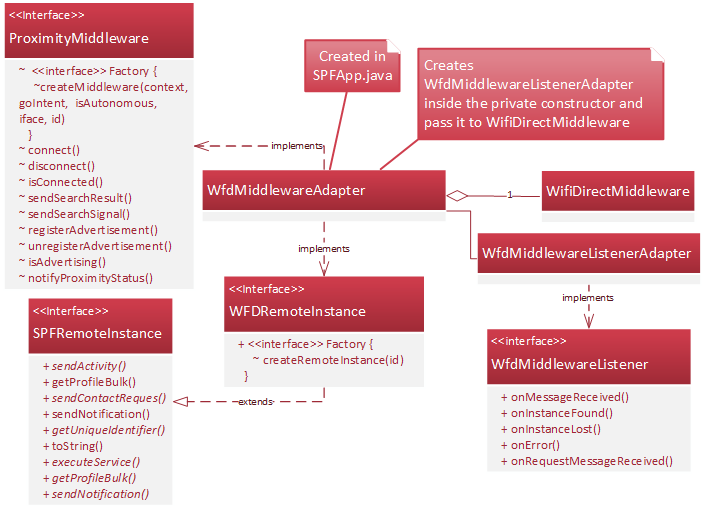
\includegraphics[scale=0.5]{./images/chap2/uml-parte1.png}
	\caption{Middleware's initial Class Diagram}
	\label{uml-part1}
\end{figure}	

\begin{figure}[thpb]
	\centering
	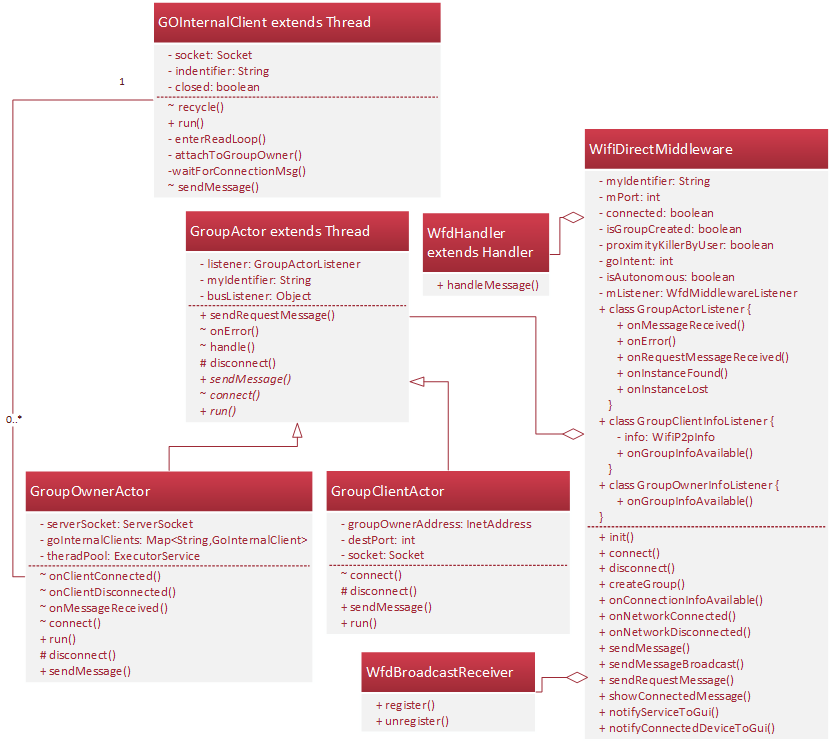
\includegraphics[scale=0.6]{./images/chap2/uml-parte2.png}
	\caption{Middleware's groups management Class Diagram}
	\label{uml-part2}
\end{figure}	


Now, I want to explain quickly the class structure of this middleware. Because there is a huge number of classes, I selected only a subset of these, as you can see in Figures \ref{uml-part1} and \ref{uml-part2}.
I cannot and I don't want to explain in details all classes and methods, because it's impossibile. Also, I don't want to repeat the same things for \textsf{GroupActor} and its subclasses. In this subsection, I want to explain some key feature of this new implementation of \textsf{WifiDirectMiddleware.java}.
In fact, there are some new important variable, like \textsf{isAutonomous} and \textsf{goIntent}. These variables are important, because chosen by the user from the UI. The first one is connected to the state of the switch ``Group Owner" and the second one to the switch ``Autonomous". 
I implemented a quick workaround to achieve this, by passing variables during the creation of the Middleware and updating these values after every change of switches. Obviously, this is not good and I'll explain why into Section \ref{conclusion}.


\section{Eternal Connect}

\emph{Eternal Connect} is a solution to restart discovery and connect phases after any network errors. This can be considered an improved version of the 	\emph{Eternal Discovery} that I used in \seqsplit{https://github.com/deib-polimi/PigeonMessanger}, because with this latest implementation, SPF will re-connect automatically trying every 15 second for 4 times. Obviously, you can configure this to achieve the best configurations. Also, you can improve \emph{Eternal Connect} in different ways to obtain also better performances during network creation, in particular on the Group Owner in Autonomous mode. All the code related to \emph{Eternal Connect} is into a single class called \textsf{EternalConnect.java}.
\emph{Eternal Connect} has two different modes:
\begin{enumerate}
	\item standard: with automatic reconnection in a loop cycle for 4 times every 15 seconds.
	\item simple: with a single automatic reconnection. If it fails, it will stop.
\end{enumerate}
These two modes are partially implemented, because I created only the necessary features. If you need a different behavior, you can simply modify \textsf{onEternalConnectUpdate} that catches \textsf{EternalConnectEvent} in \textsf{WifiDirectMiddleware.java}. \textsf{EternalConnect.java} is a singleton class with these important public methods:
\begin{itemize}
	\item \textsf{eternalConnect()}: start the \emph{EternalConnect} as you can see in Listing 	\ref{eternalConnect}.
	\item \textsf{onNetworkDisconnected()}: if a device isn't a GO in Autonomous mode, this method will restart the \emph{Eternal Connect}, otherwise it will post an \textsf{EternalConnectEvent} to specify the ``simple reconnection" mode;
	\item \textsf{onConnectFailed()}: called when Wi-Fi Direct fails during the connection procedure, to restart the \emph{Eternal Connect} in standard mode;
	\item \textsf{onGroupCreationFailed()}: called when Wi-Fi Direct fails during the group creation procedure, to restart the \emph{Eternal Connect} in ``simple mode";
	\item \textsf{eternalCompletedSuccessfully()}: to complete the procedure, because the connection is established.
\end{itemize}


\begin{lstlisting}[caption={eternalConnect() method},label=eternalConnect, language=Java]
void eternalConnect(boolean proximityKilledByUser) {
  killScheduler();
  scheduler = Executors.newScheduledThreadPool(1);
    final Runnable runnable = new Runnable() {
      public void run() {
        if (proximityKilledByUser) {
        	  killScheduler();
          eternalCounter = 0;
          return;
        }	
		if (eternalCounter > MAX_ETERNAL_COUNT) {
          killScheduler();
          eternalCounter = 0;
        } else {
        	  //post EternalConnectEvent.NEW_EC_CYCLE
          eternalCounter++;
        }
	}
};

final ScheduledFuture<?> eternalHandle =
  scheduler.scheduleAtFixedRate(runnable, 
    10, 15, TimeUnit.SECONDS);
  scheduler.schedule(new Runnable() {
    public void run() {
      eternalHandle.cancel(true);
    }
  }, 15, TimeUnit.SECONDS);
}
\end{lstlisting}


\section{Wi-Fi Direct's known issues}

In this section i want to create a list with some of the known issues of Wi-Fi Direct protocol on Android devices.
\begin{itemize}
	\item There are random errors when you are trying to establish a connection. In most of the cases, to fix this problem you must kill the Wi-Fi Connection manually.
	\item The discovery procedure is absolutely unreliable. Sometime a device can't discover other devices without any reason and the only way to fix this problem is a stop, followed by a restart of the discovery procedure.
	\item Connection between different devices with different Android versions and manufacturers can be unstable.
	\item The most important problem in SPF2 is related to autonomous group join operations. Because, if a device want to join to a previously created group, it should ask to the GO of this group to join in. In Android API there isn't this concept (in wpa\_supplicant yes, obviously), but there is the standard \textsf{connect()} method. This is not a problem, instead the real problem is that if a device want to join, on the GO will appear a popup. If the GO accept the join procedure, the connection can be completed. This process can't be automated and always requires a user interaction. Also, for absolutely inexplicable reasons, when the connection with a third device starts, the entire group can be destroyed to try to recreate it quickly. This is a famous problem that you can found everywhere on stackoverflow. At the moment there aren't any solutions. If you want to use wpa\_supplicant from command line this problem never happens, this implies that is caused by the Android implementation of Wi-Fi Direct. Also, the main consequence related to this problem is that sometime the group won't be recreated, caused by fails during connection or discovery problems. To be able to create a group of three devices with SPF2, you should try some times to obtain the desired result. This is a huge Android's implementation issue, impossibile to fix, at the moment.
\end{itemize}



\chapter{New Material Design GUI}
\label{gui}

In this short chapter i'll show the main improvements to the GUI.
Mainly, I used all available elements into the support library and I replaced the Holo Theme with ``Theme.AppCompat.Light.NoActionBar" to mimic the Material Theme. Also, when necessary, I used the Compat element, like CompatButton and so on to show the same element in different Android's versions. When possibile I replaced unofficial libraries or old component with the new Google Design support library, for example to crete tab layouts. 

\begin{figure}[thpb]
\centering
\begin{minipage}[b]{0.4\textwidth}
	\centering
	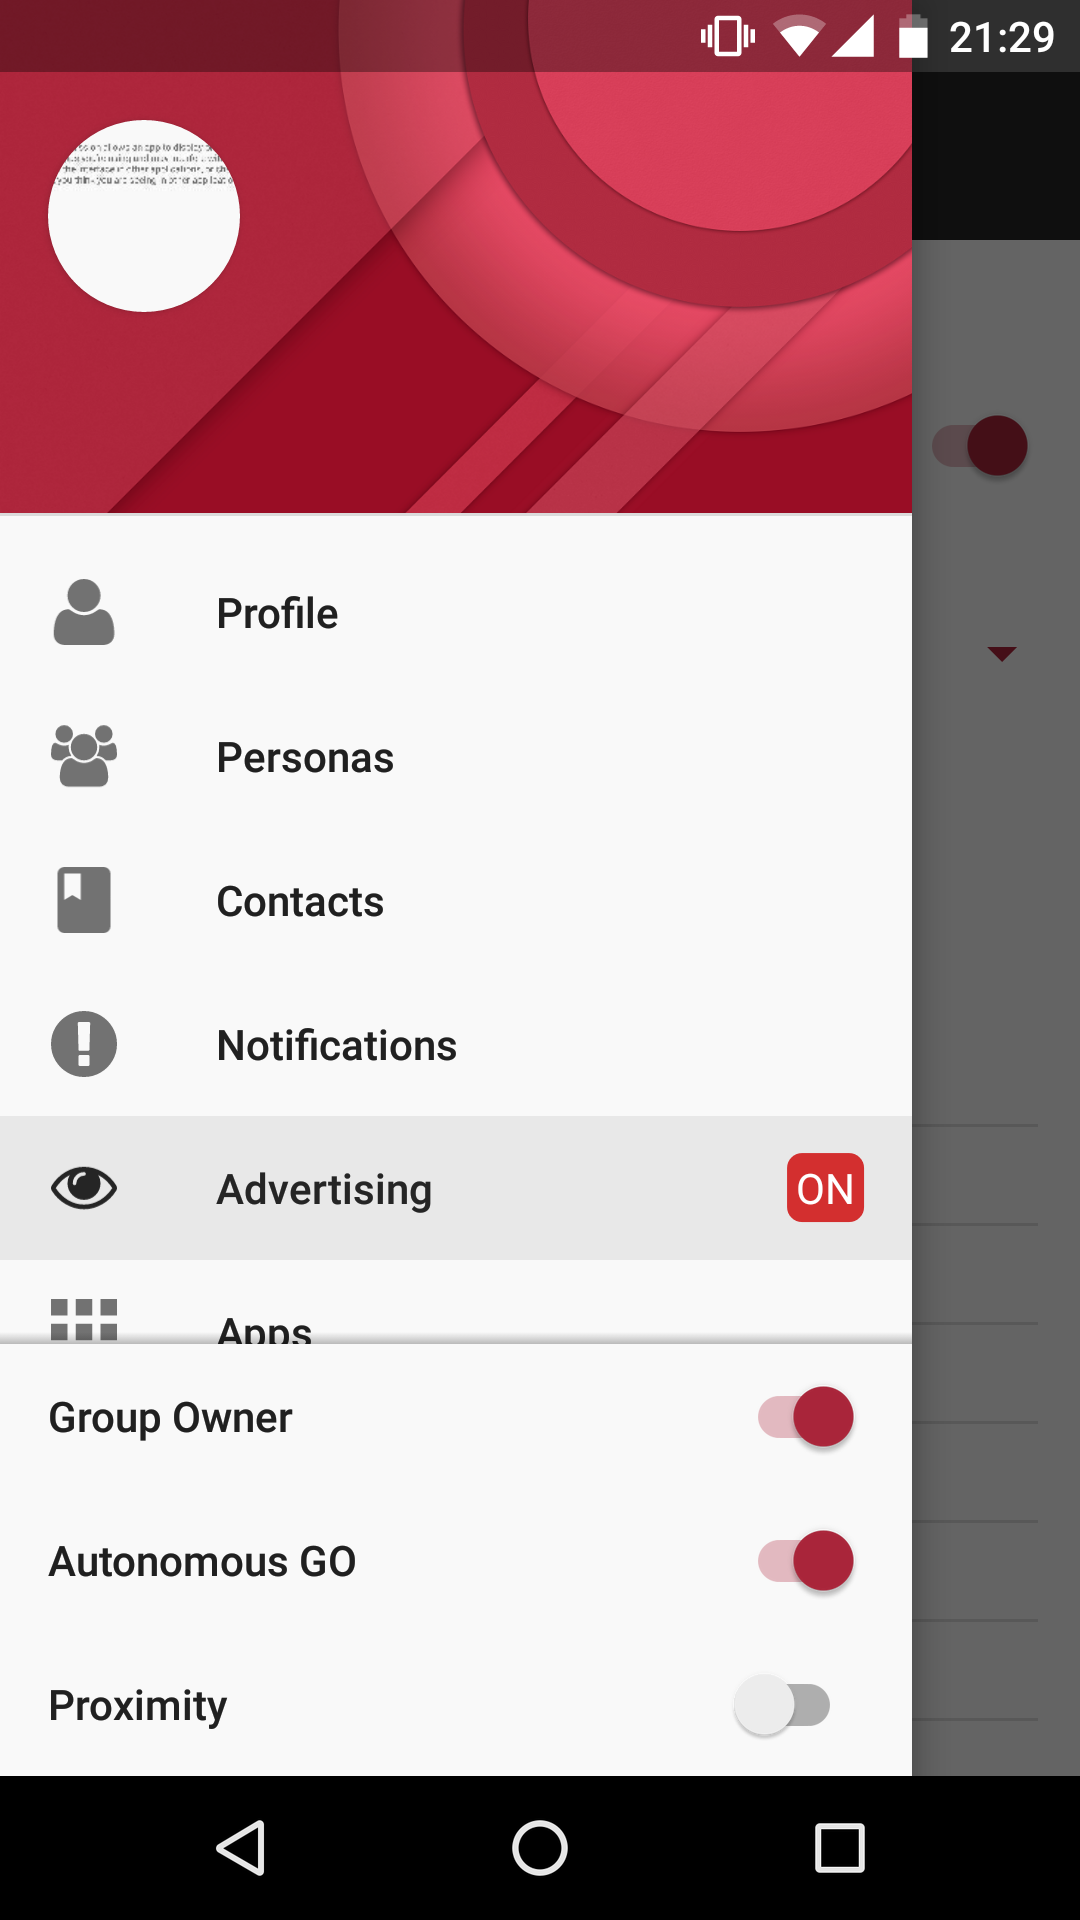
\includegraphics[scale=0.1]{./images/chap3/drawer.png}
	\caption{Drawer}
	\label{fig:drawer}
\end{minipage}
\hfill
\begin{minipage}[b]{0.4\textwidth}
	\centering
	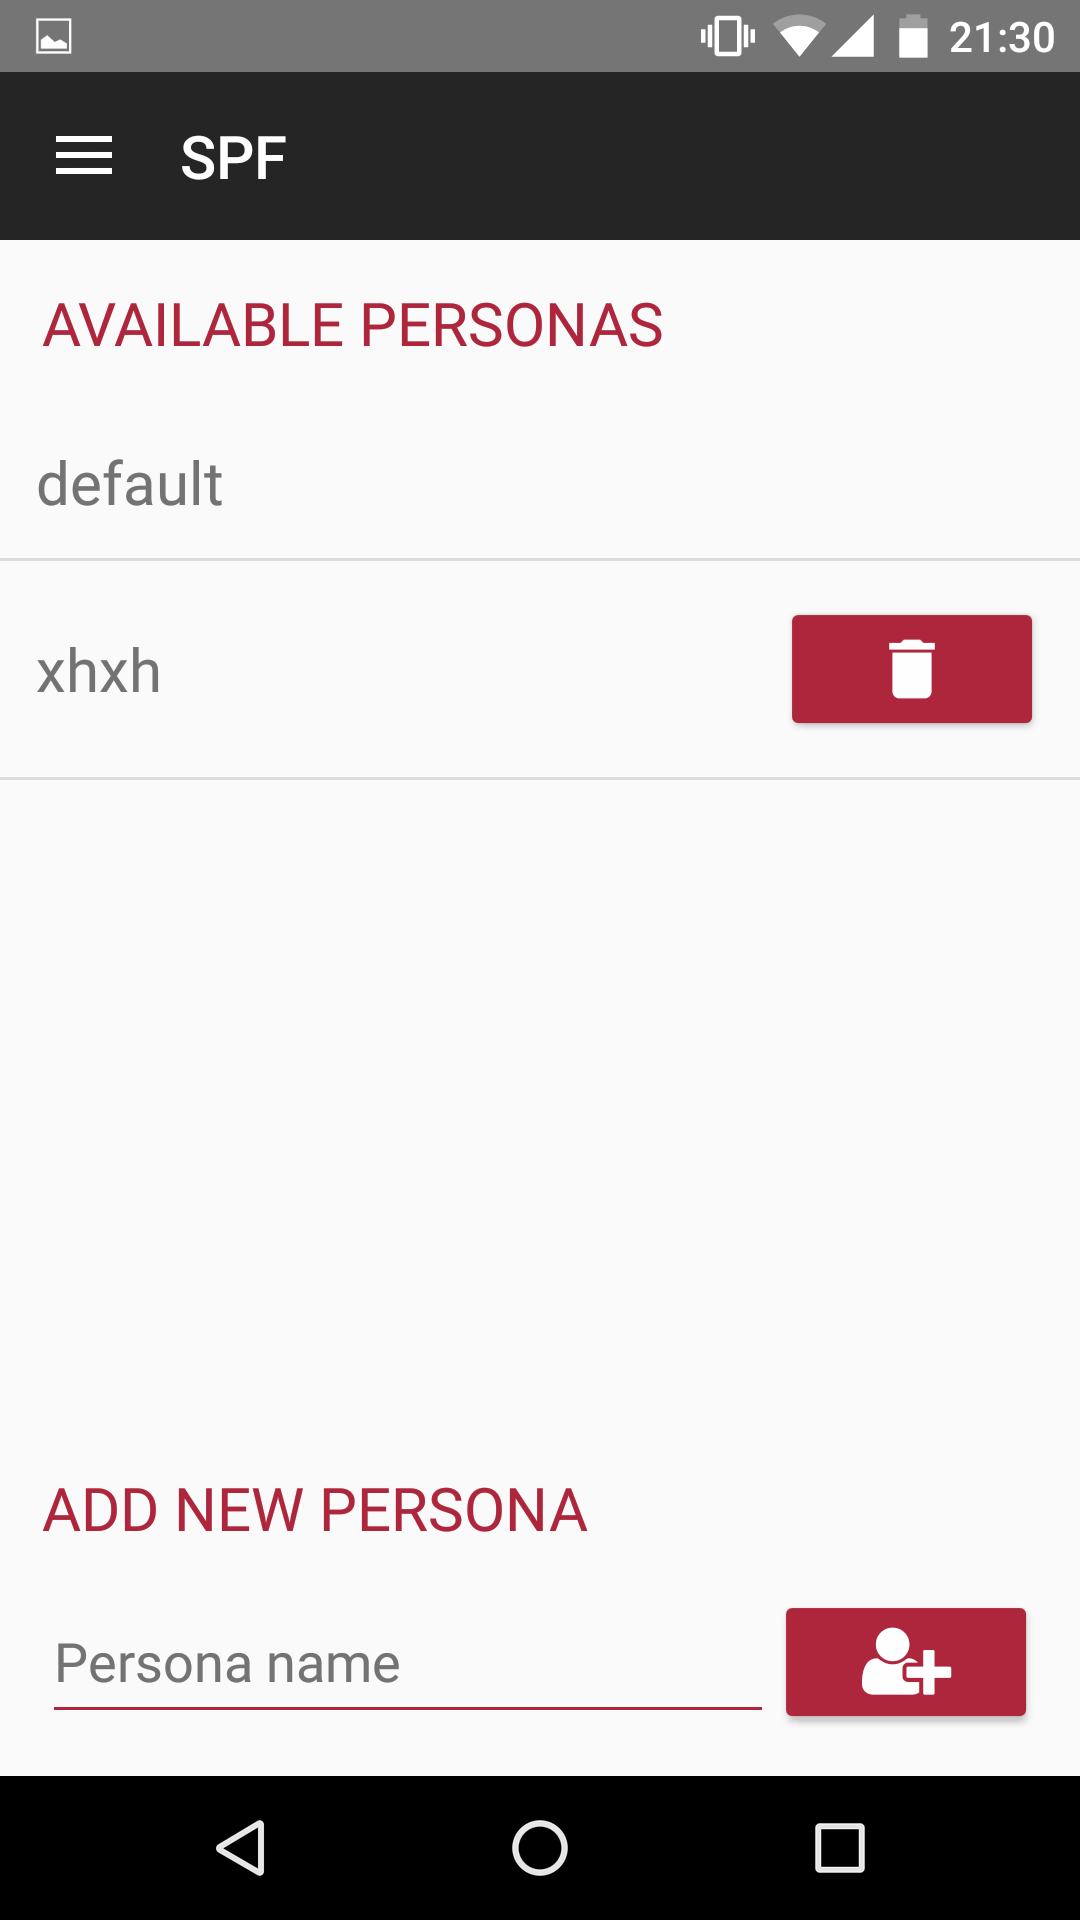
\includegraphics[scale=0.1]{./images/chap3/bottom_iconics.png}
	\caption{Buttons with Iconics}
	\label{fig:buttom-iconics}
\end{minipage}	
\end{figure}	

I applied all this updates to all SPF's apps. Also, I implemented the Material Drawer using a custom unofficial library available on GitHub, created by Mike Penz. The idea was to build a cool Material Drawer very quickly without to implement manually some annoying features. The result is in Figure \ref{fig:drawer}. In addition, I used Iconics library to add vector icons to buttons, toolbar and to the drawer's items, as in Figure \ref{fig:buttom-iconics}.

\begin{figure}[thpb]
\centering
\begin{minipage}[b]{0.4\textwidth}
	\centering
	
\includegraphics[width=\textwidth]{./images/chap3/header.png}
	\caption{Header}
	\label{fig:header}
\end{minipage}
\hfill
\begin{minipage}[b]{0.4\textwidth}
	\centering
	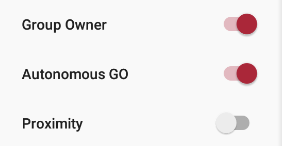
\includegraphics[width=\textwidth]{./images/chap3/switches.png}
	\caption{Drawer's switches}
	\label{fig:switches}
\end{minipage}	
\end{figure}


\begin{figure}[thpb]
	\centering
	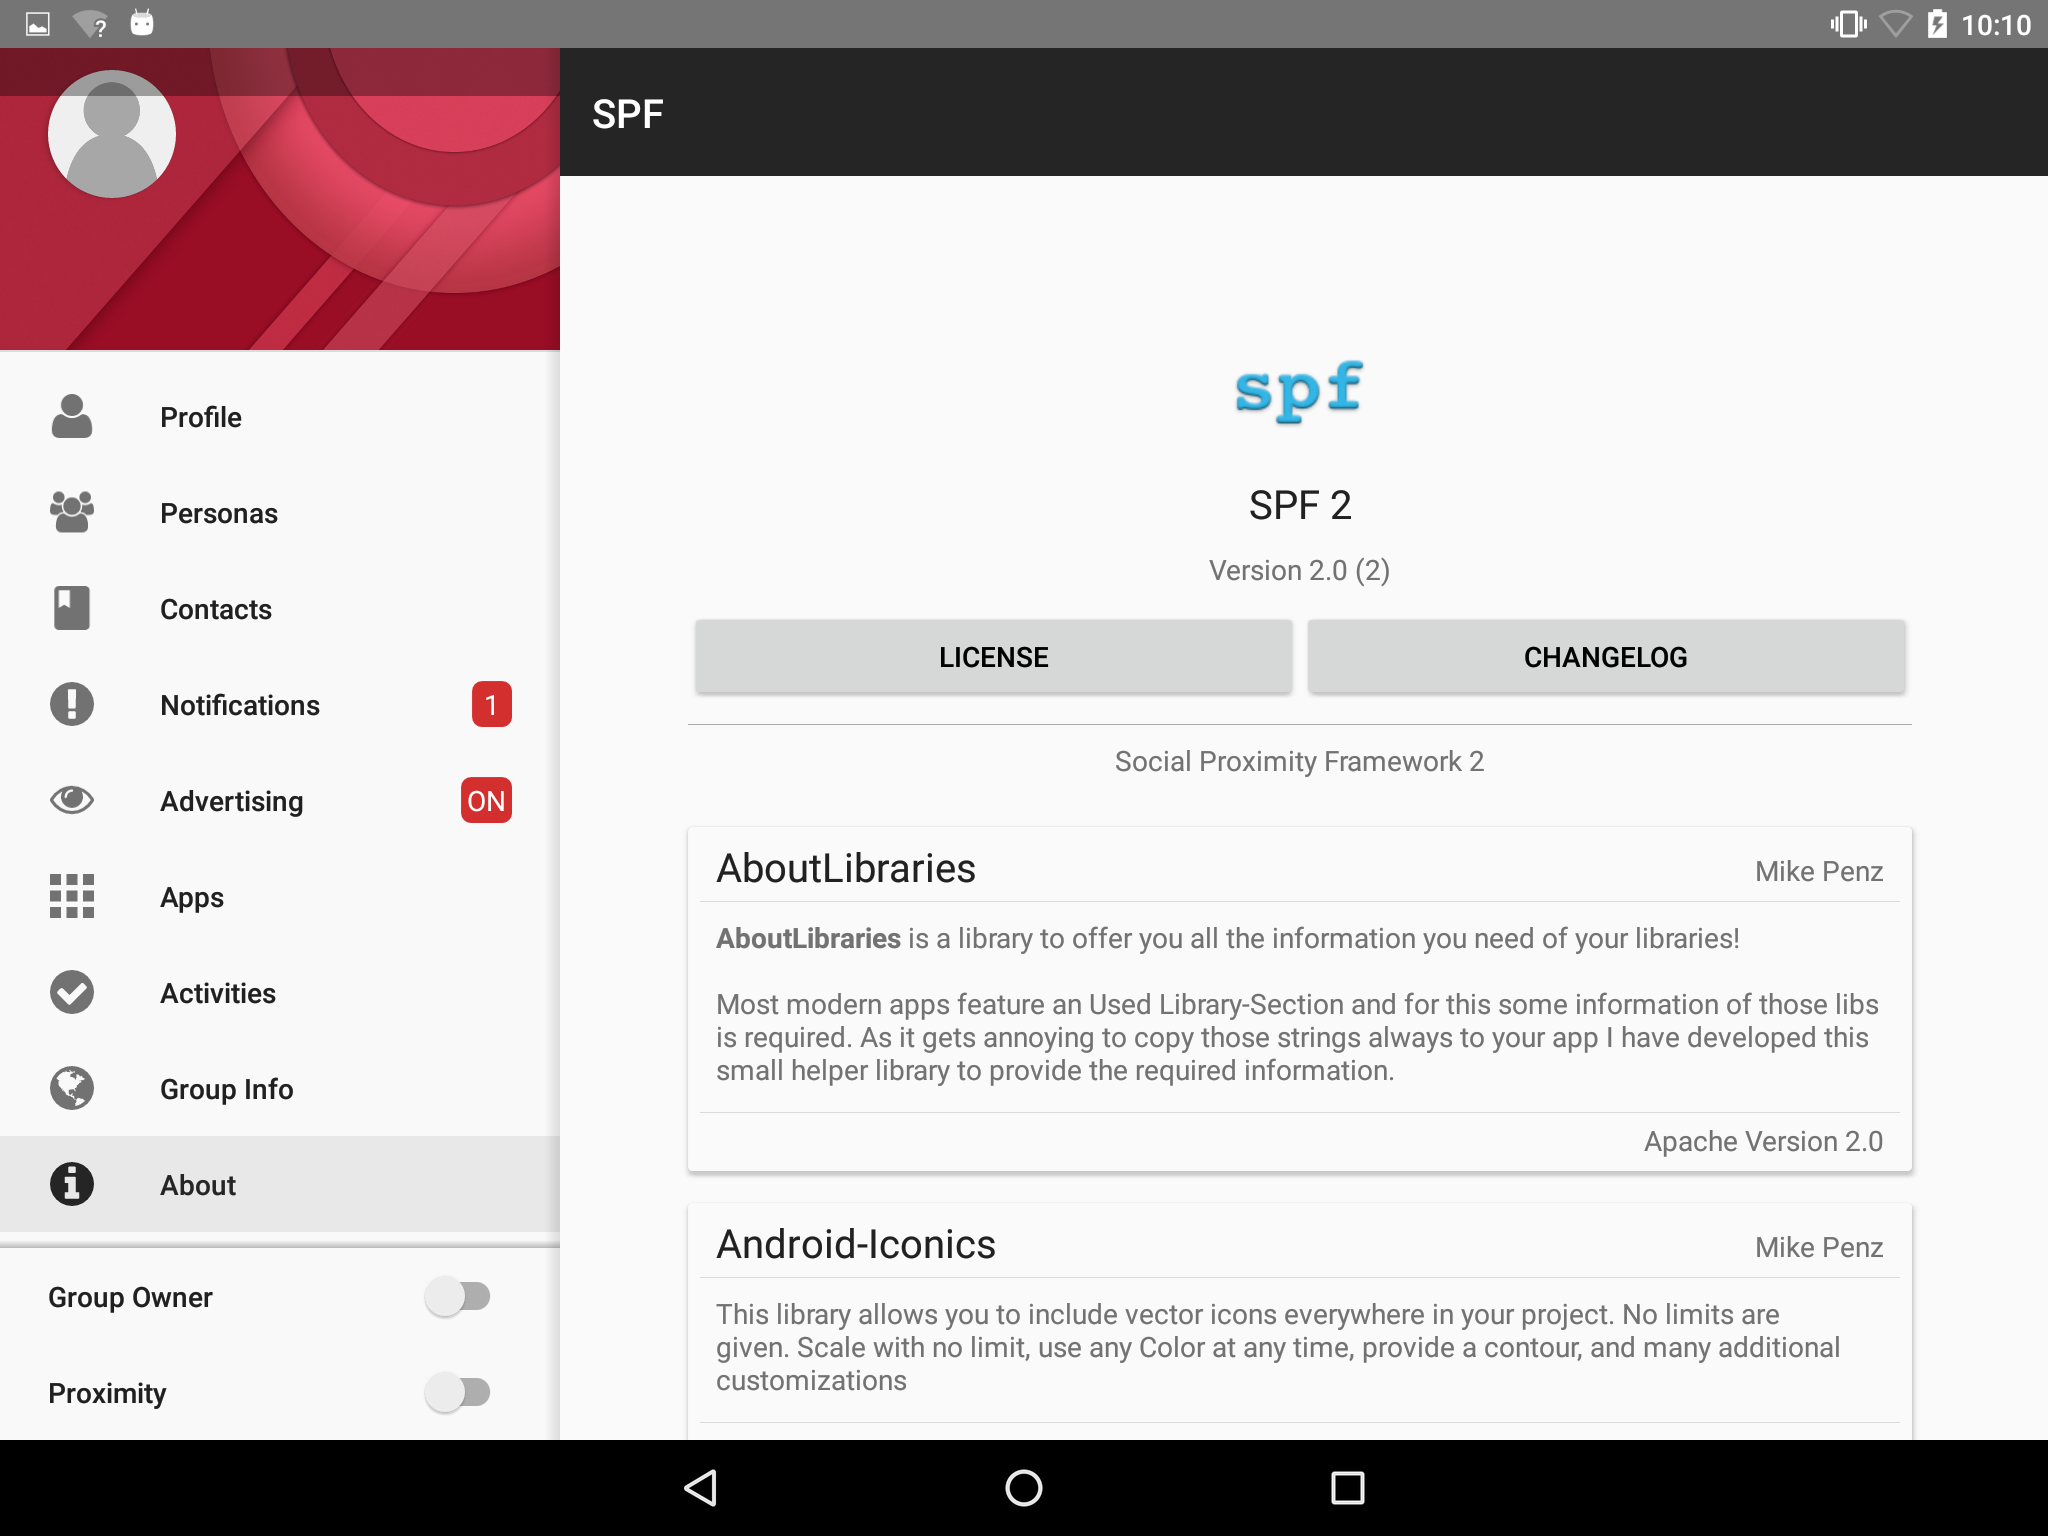
\includegraphics[scale=0.15]{./images/chap3/about_fragment.png}
	\caption{About Fragment}
	\label{fig:about}
\end{figure}	


As you can see, i added a Header with an image and the profile photo (Figure \ref{fig:header}) and a Sticky Footer into the drawer, with switches (Figure \ref{fig:switches}). Also, I added two new items: Group Infos and About. The first one selects a fragment with the available services and the connected devices. This is not necessary to users, but it very useful during development to understand if a device is still connected or if there are problems related to Wi-Fi Direct. The second one is a simple about page of SPF, created with a library that compose this Activity scanning the libraries and dependencies used inside this application, automatically, as in Figure \ref{fig:about}.

\begin{figure}[thpb]
	\centering
	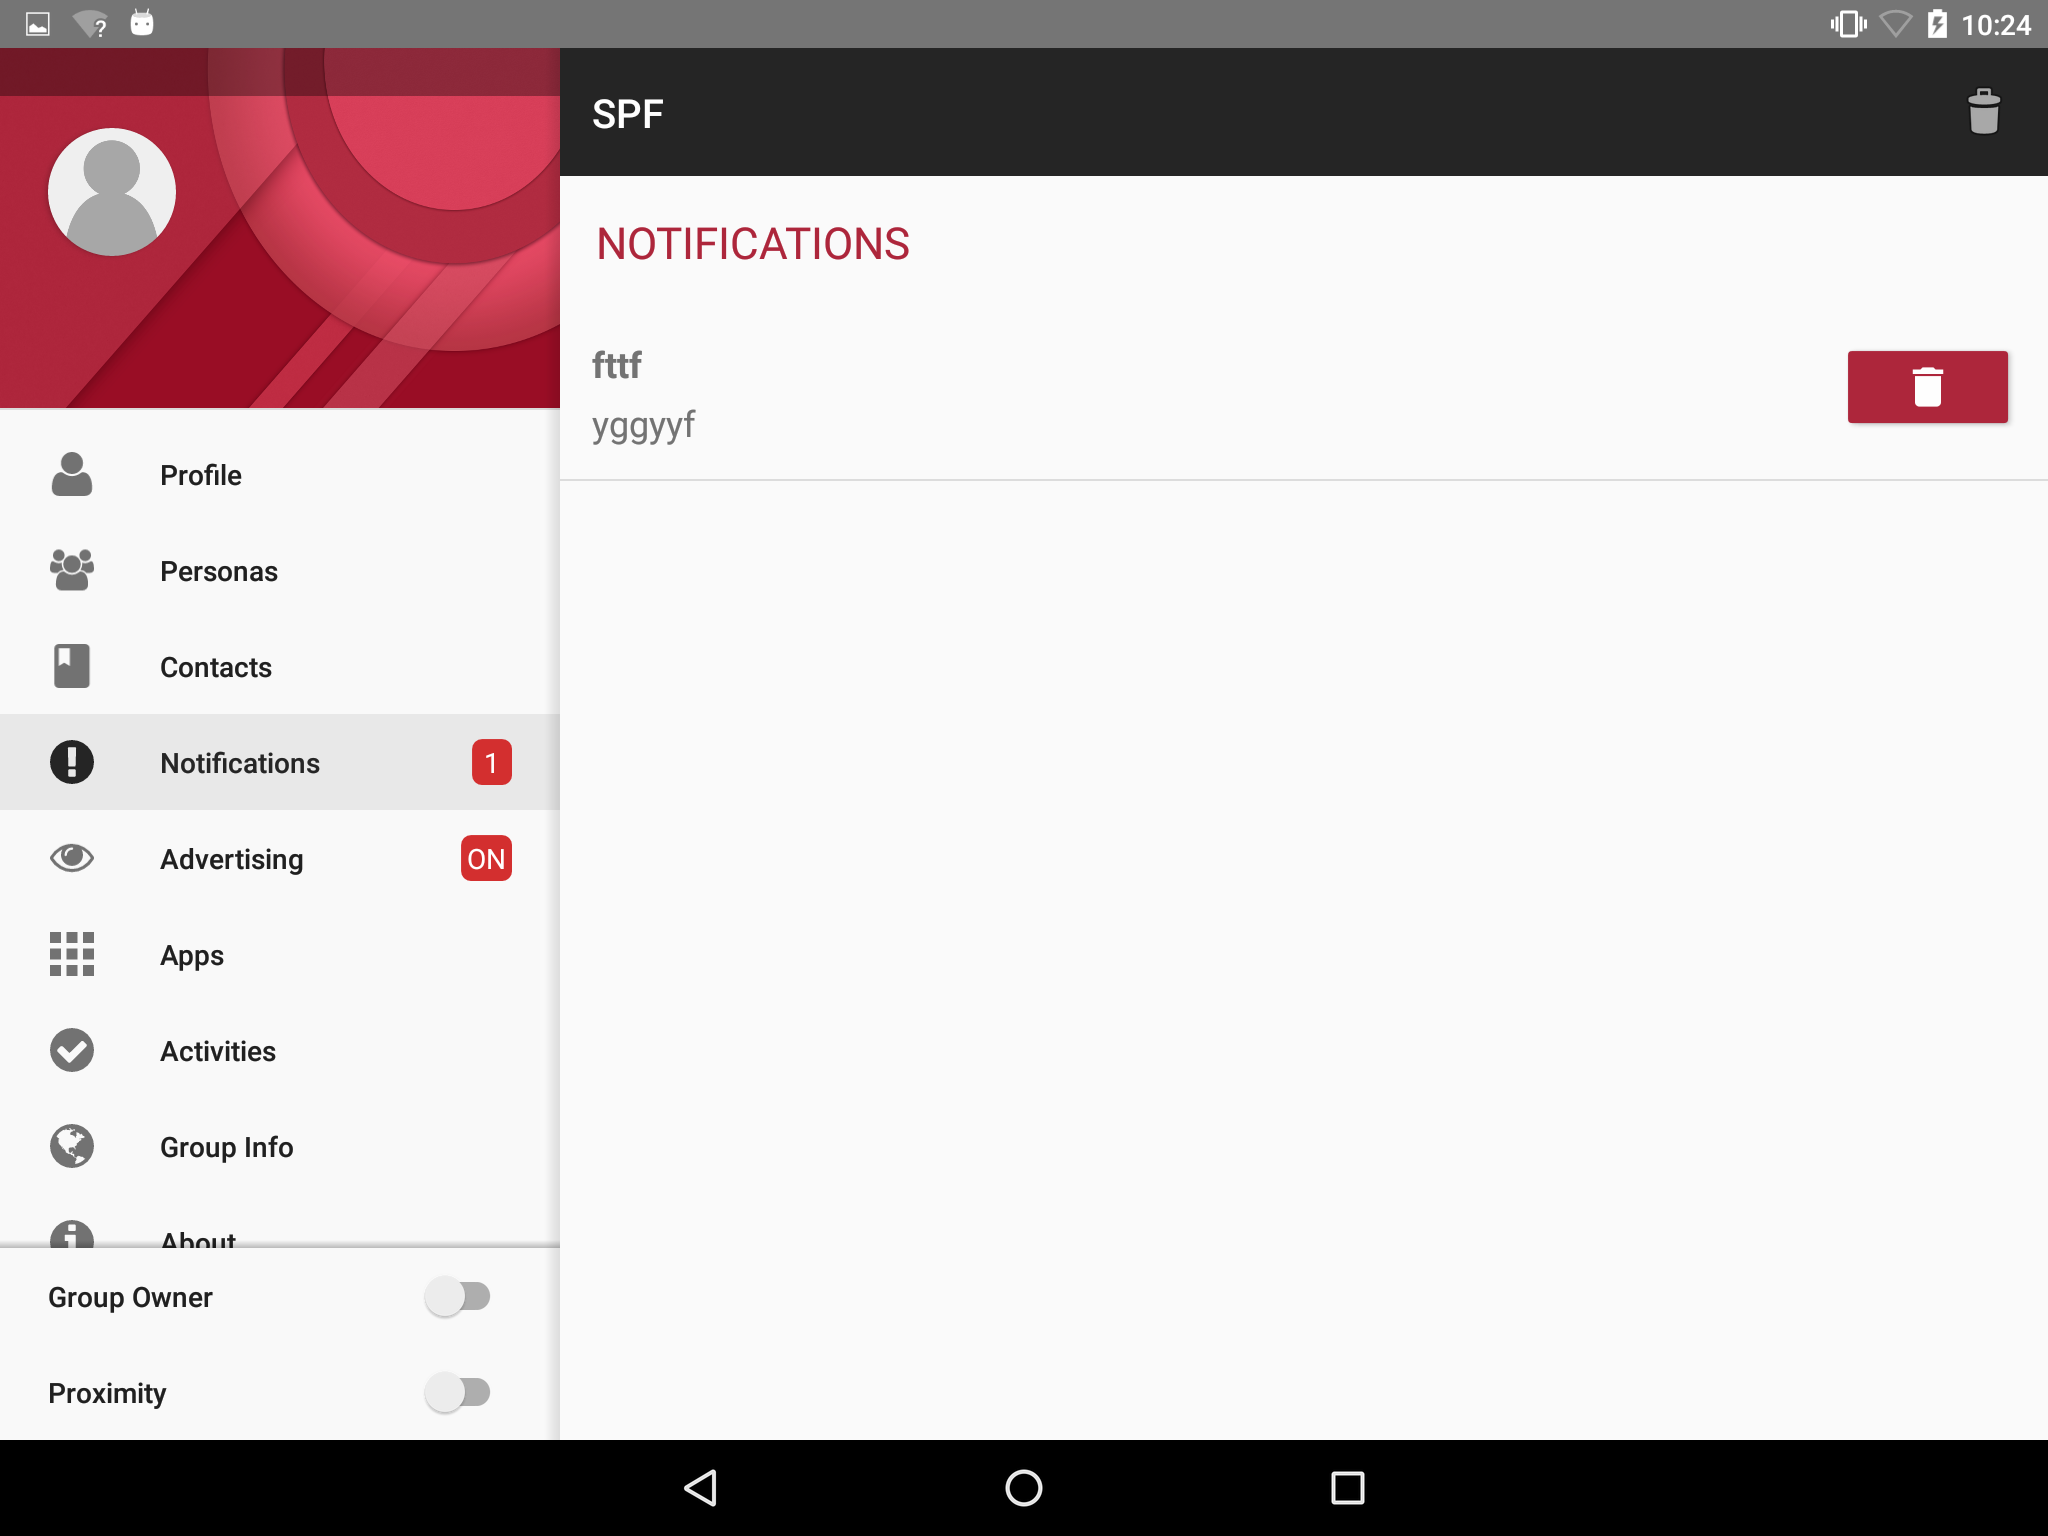
\includegraphics[scale=0.15]{./images/chap3/tablet1.png}
	\caption{Multi-pane layout}
	\label{fig:tablet1}
\end{figure}	


After this quick explanation i want to explain one of this features, i.e. the Material Drawer, in particular how to reuse the same Drawer for smartphone and Tablets to create a Multi-pane layout, as in Figure \ref{fig:tablet1}.

In Listing \ref{lst:multipane} there is a shorter version of the code that I used to create the drawer. All the method's invocations are chained, because every method returns always the same object, DrawerBuilder.


\begin{lstlisting}[caption={DrawerBuilder creations},label=lst:drawerbuilder, language=Java]
drawerBuilder = new DrawerBuilder()
  .withActivity(this)
  .withAccountHeader(headerResult)
  .withHasStableIds(true)
  .withToolbar(toolbar)
  .addDrawerItems(
    new PrimaryDrawerItem().withName(mSectionNames[0])
      .withIdentifier(0).withIcon(FontAwesome.Icon.faw_user),
    	(...)
  )
  .withOnDrawerItemClickListener(drawerItemClickListener)
  .withSavedInstance(savedInstanceState);
\end{lstlisting}


And finally, in Listing \ref{lst:multipane} I added the code to reuse the MaterialDrawer to create a Multipane layout. The trick is to the view obtained from the drawer to the viewGroup related to the layout's element, a simple FrameLayout that I called \textsf{nav\_tablet}. Obviously you need two layouts, one for smartphones and one for tablet. In the first case you must use a DrawerLayout, in the second one you could simply use a FrameLayout.


\begin{lstlisting}[caption={Reuse Drawer for Multi-pane layout},label=lst:multipane, language=Java]
if (tabletSize) {
  //if tablet create a multipane layout
  drawer = drawerBuilder.buildView();
  ((ViewGroup) findViewById(R.id.nav_tablet))
    .addView(drawer.getSlider());
} else {
  //on smartphones i want to show the hamburger icon
  if (getSupportActionBar() != null) {
    getSupportActionBar().setDisplayHomeAsUpEnabled(false);
  }
  drawerBuilder.withActionBarDrawerToggle(true);
  drawerBuilder.withActionBarDrawerToggleAnimated(true);
  drawer = drawerBuilder.build();
  drawer.getActionBarDrawerToggle()
    .setDrawerIndicatorEnabled(true);
}
\end{lstlisting}



\chapter{Changelog}
\label{changelog}

In this section i want to write a list with all major changes made in SPF2 compared to SPF1. This can be considered as a complete changelog of SPF2 and its demo applications.

\subsection*{Changelog SPF}
\begin{enumerate}
	\item project moved from Eclipse to Android Studio.
	\item SPFShared and SPFLib are remote dependencies into a maven repository for external apps, but at the same time they are local projects for SPF.
	\item created a gradle task to upload dependencies into a Sonatype Nexus Server.
	\item updated to Lollipop/Marshmallow Material Design using support libraries.
	\item code cleanup using \emph{Butterknife}, \emph{Otto} and \emph{Project Lombok}. Also, improved architecture removing cyclic dependencies.
	\item completely removed \emph{AllJoyn/AllSeen}'s middleware. SPF2 has a pure Wi-Fi Direct Middleware implementation.
	\item notification into \emph{Notification Drawer} updated with a custom layout (using \emph{RemoteViews}) adding an "X" button to stop the \emph{Proximity Service}.
	\item fixed BUG ID=0: crashes related to profile image. Now I'm using \emph{android-crop} by \emph{soundcloud} to pick and cut images. Also, I added another library to create a \emph{circular image view}.
	\item added \emph{Travis CI} to the GitHub repository.
	\item fixed BUG ID=2: problem when I'm trying to save profile's fields. I replaced the listener with a \textsf{TextWatcher}.
	\item fixed BUG ID=9: when \textsf{SPFCouponingClient} is closed, \textsf{SPFFramework} receives and saves coupons ignoring my filter. To fix this problem, I changed the filter to use the db, instead of the data saved in memory.
	\item huge code refactoring and design improvements into Wi-Fi Direct Middleware.
	\item fixed BUG ID=11: NullPointerException in \textsf{GroupActor}.
	\item implemented a quick workaround to specify \emph{go\_intent} and \emph{autonomous mode} from the GUI, using switches.
	\item fixed BUG ID=12: ``service is null" in middleware.
	\item performance improvements for group creation's procedure into the middleware.
	\item fixed Bounjour protocol logic into the middleware.
	\item added Toast notification to explain the connection status.
	\item fixed BUG ID=14: NullPointerException (but I don't remember where).
	\item using the unique identifier I created a quick logic to tell to clients if a device is a GO or not. In fact, now GOs have ids that start with the ``AP" prefix.
	\item fixed BUG ID=15: implemented a logic to connect only to ``AP" devices.
	\item fixed BUG ID=16: related to ID=15 but isolated into \textsf{ServiceList} class.
	\item implemented Wi-Fi Direct's \emph{Autonomous Mode} for GOs.
	\item implemented a new logic to manage in a better way the selection of Socket's ports.
	\item log system updated and added code to catch all exceptions in the middleware.
	\item increased connection's timeout on clients to reduce problems during the connection procedure.
	\item fixed BUG ID=17: in a specific part of the middleware, \textsf{socket.close()} were called by the UI Thread causing a caught and ignored exception. Fixed using \emph{Otto}'s events to create asynchronous calls.
	\item implemented a complete Event's hierarchy used for Otto bus.
	\item completely redesigned \textsf{GroupActor} and its subclasses. The superclass is a Thread and all subclasses implement \textsf{run()} and other abstract methods.
	\item removed \textsf{ServerSocketAcceptor} and moved into \textsf{GroupOwnerActor}.
	\item removed cyclic dependency between \textsf{WifiDirectMiddleware} and \textsf{WFDBroadcastReceiver} using \emph{Otto}'s events.
	\item implemented Wi-Fi Direct Group's management into Wi-Fi Direct middleware (not really stable, but the problem is related to the Android's implementation of this protocol).
	\item fixed BUG ID 18: Android 6.0 Marshmallow changed the permission policy. For this reason, I implemented a workaround to guide the user to enable a specific feature, required by external apps to interact with the framework.
	\item \textsf{SPFApp} updated with the new Google Design library, for example to create Tabs.
	\item fixed BUG ID=20: added a default photo profile.
	\item fixed BUG ID=21: fixed small bug related to tabs.
	\item implemented \textsf{Eternal Connect} in a singleton class. It's an evolution of the \textsf{Eternal Discovery} that I previously created for \emph{Pigeon Messenger} (\seqsplit{https://github.com/deib-polimi/PigeonMessanger}). \textsf{Eternal Connect} is able to discovery and connect automatically to nearby devices.
	\item added two new fragments: \textsf{GO Infos} and \textsf{About}. The first shows all informations about services and connection status, the second one is an about page.
	\item completely rewritten the navigation drawer using \textsf{MaterialDrawer} and \textsf{Iconics} to create a modern GUI. Also, I reused the same code to update the \emph{Multi-pane layout} for tablets.
\end{enumerate}

\subsection*{Changelog SPFCouponingProviderDemo}
\begin{enumerate}
	\item moved outside the main repository with the framework.
	\item updated to Lollipop/Marshmallow Material Design using support libraries.
	\item fixed BUG ID=3: crashes related with profile image. Now i'm using \emph{android-crop} by \emph{soundcloud} to pick and cut images. Also, I added another library to create \emph{circular image view}.	
	\item added \emph{Travis CI} to the GitHub repository.
\end{enumerate}

\subsection*{Changelog SPFCouponingClientDemo}
\begin{enumerate}
	\item moved outside the main repository with the framework.
	\item updated to Lollipop/Marshmallow Material Design using support libraries.
	\item fixed BUG ID=3: crashes related with profile image. Now i'm using \emph{android-crop} by \emph{soundcloud} to pick and cut images. Also, I added another library to create \emph{circular image view}.	
	\item added \emph{Travis CI} to the GitHub repository.
	\item fixed BUG ID=4: coupons received multiple times, adding multiple times the same element to the list.
	\item fixed BUG ID=5: added a method to delete ``interests" in \textsf{SPFApp} directly from Couponing app recycling existing methods.
	\item fixed BUG ID=6: \textsf{CouponCreationActivity} has leaked \textsf{ServiceConnection}.
	\item fixed BUG ID=7: app crashes when i'm trying to add categories.
\end{enumerate}

\subsection*{Changelog SPFChatDemo}
\begin{enumerate}
	\item moved outside the main repository with the framework.
	\item updated to Lollipop/Marshmallow Material Design using support libraries.	
	\item added \emph{Travis CI} to the GitHub repository.
\end{enumerate}

\chapter{Conclusions, limitations and future work}
\label{conclusion}

SPF2 is the new major release of SPF. In this document, I explained the main changes made to this software. In particular, I updated the entire project to Android Studio, moving dependencies into Maven repositories. Also, I changed the theme to Material Design, using support libraries and other third party softwares. SPF2 is fully compatibile with Android Lollipop (5.x) and Marshamallow (6.0). I removed \emph{AllJoyn} and improved the Wi-Fi Direct Middleware to be able to manage group of devices.

However, there are some open issues and improvements that you can do to SPF. To be able to extend this software in an interesting way, you should completely redesign the communication between SPFApp and its submodules. If you'll move SPFApp into another project and you'll implement a remote communication between SPFApp and the framework exposing methods, you will really able to extends SPF to more interesting scenarios.

Also, the first implementation of SPF completely ignored the different roles of nodes into a network (like Master/Slave or Group Owner/Client). For timing constraints, I chose a quick solution to archive this, adding switches into the GUI and send their states to the middleware. This solution is temporary, because it is terrible from the design point of view. If you have enough time, you should really extract \textsf{SPFApp} from the main Android Studio's project. I mean that, \textsf{SPFFramework} (with \textsf{SPFShared}, \textsf{SPFLib} and \textsf{SPFWFDMiddleware}) should be a library available in Maven, and demo applications could import this framework using a dependency into their \textsf{build.gradle}'s files. \textsf{SPFApp} should be an optional app to configure \textsf{SPFFramework} using remote communication. In this way, you can simply reuse the same framework for GOs and Clients, for example Shop manager and his customers, without to release on the market an application that can creates other GOs. Also, in this way you can remove the terrible workaround that I obliged to implement to build this new major release.

I repeat, the main focus for the next versions should be the extraction of \textsf{SPFApp} from the main project, creating a standalone project with remote calls to the previous one.



\section*{Open issues}
Obviously, there are other open issues. I decided to write all known problems and suggestions here.
\begin{enumerate}
	\item If discovery phase fails, create a temporized system to restart it automatically.
	\item When SPF enters in \textsf{onConnectionInfoAvailable()}, start a timer on the client. At the end of the countdown, if this device isn't connected to the GO it should restart the discovery phase.
	\item Refactor \textsf{MainActivity.java} to reduce codelines.
	\item Updates the proximity switch in the GUI accordingly to the service status. For example, when Eternal Connect is working, you should update the switch. I suggest to use \emph{Broadcast receivers} (not \emph{Local}, but \emph{Remote} declared into the \textsf{AndroidManifest.xml}). Use \textsf{GroupInfosFragment} as an example.
	\item Remove all \emph{ListViews} and replace they with \emph{RecyclerView}. Use \textsf{GroupInfosFragment} as an example.
	\item Fix Tab positioning for tablets/smartphones. You should find a way to display centered tabs that fill the entire screen width, but with text on a single line. Your solution should work also during screen rotation.
	\item Improve the \emph{standard mode} into the Wi-Fi Direct Middleware.
	\item Replace \emph{materialtabstrip library} with the official version included into \emph{Design support library} by Google, either for \textsf{CouponingProvider} or \textsf{CouponingClient}.
	\item Replace \emph{multiselection library} in \textsf{CouponingProvider} and \textsf{CouponingClient} with an official version.
	\item Update the \emph{profile identifier} accordingly to the device role into the network (GO or Client). Remember that I'm using the ``AP" prefix to identify GOs.
	\item Check if Wi-Fi is enabled during start-up.
	\item Rewrite the entire \textsf{ProfileFragment} GUI using \emph{RecyclerView} and statical xml's layout to simplify the code.
\end{enumerate}


%\cleardoublepage
% ---- Bibliography ----
%\addcontentsline{toc}{chapter}{Bibliography}
%\bibliographystyle{plain}
%\bibliography{bibliography}
%\nocite{*}

%\appendix

% ---- Page footer setup ----
\pagestyle{fancy} 
\fancyfoot{}                                               
\renewcommand{\chaptermark}[1]{\markboth{\appendixname\ \thechapter.\ #1}{}} 
\renewcommand{\sectionmark}[1]{\markright{\thesection.\ #1}}         
\fancyhead[LE,RO]{\bfseries\thepage}
\fancyhead[RE]{\bfseries\leftmark}    
\fancyhead[LO]{\bfseries\rightmark}     
\renewcommand{\headrulewidth}{0.3pt} 

%\chapter{Appendix 1 title}
\label{appendiceA}
\thispagestyle{empty}

\noindent 
Documentation dabsbdasd sahdjasjdas dasdhasjdajsd

\end{document}